\documentclass[a4paper,titlepage,fleqn,12pt]{article}

\usepackage[utf8]{inputenc}
\usepackage[T1]{fontenc}
\usepackage[english]{babel}
\usepackage{color}
\usepackage{float}
\usepackage{fancyvrb}
\usepackage{amssymb}
\usepackage{amsmath}
\usepackage{listings}

\usepackage{comment}

\usepackage{graphicx}
\usepackage{epstopdf}
\usepackage{ulem}
\usepackage{pdfpages}

\setcounter{secnumdepth}{1}
\setcounter{tocdepth}{1}

\DeclareGraphicsExtensions{.png}

\definecolor{dkgreen}{rgb}{0,0.45,0}
\definecolor{gray}{rgb}{0.5,0.5,0.5}
\definecolor{mauve}{rgb}{0.30,0,0.30}

\lstset{frame=tb,
  language=Java,
  aboveskip=3mm,
  belowskip=3mm,
  showstringspaces=false,
  columns=flexible,
  basicstyle={\small\ttfamily},
  numbers=left,
  numberstyle=\footnotesize,
  keywordstyle=\color{dkgreen}\bfseries,
  commentstyle=\color{dkgreen},
  stringstyle=\color{mauve},
  frame=single,
  breaklines=true,
  breakatwhitespace=false,
  tabsize=1
}


\begin{document}

\begin{titlepage}
	\begin{center}
	
\includegraphics[scale=1.5,page=7]{sdu_logos.pdf}~\\[0.5cm]
	\textsc{\Large{Syddansk Universitet - Mærsk Mc-Kinney Møller Institutet}} \\[0.2cm]
	\rule{12cm}{1pt} \\[0.4cm]
	{ \huge \bfseries Interaktion og interaktionsdesign, efterår 14, Projekt del 1 \\[0.4cm] }
	\rule{12cm}{1pt} \\[1.5cm]
	
	\begin{minipage}{0.4\textwidth}
		\begin{flushleft} \large
			\textit{Author:}\\
			Morten Rovelt Hansen\\
			Brian Pedersen\\
			Steven Gøhler\\
		\end{flushleft}
	\end{minipage}
	\begin{minipage}{0.4\textwidth}
		\begin{flushright} \large
			\textit{Supervisor:} \\
			Jess Uhre Rahbek
		\end{flushright}
	\end{minipage}
	
	\vfill
	
	{\large Oktober 10, 2014}
	\end{center}
	\newpage
\end{titlepage}

\tableofcontents
\newpage

\section{Problemfelt}

\subsection{Hvad vi vil lave}
Vi vil udarbejde en hjemmeside, der gør det nemt og brugervenligt for en jobsøgende / kommende jobsøgende, at oprette og opdaterer en online-portfolie, der er nem, hurtig og let tilgængelig at præsenterer for en arbejdgiver eller bruger.

\subsection{Antagelser}
En antagelse kunne være at hjemmesiden ikke appelerer til alle erhvervsmæssige retninger, men mest af alt kan være brugbar for folk i kreative erhverv medgør. Det ville mest være henvist til folk i mode/design/foto verdenen, da det nemme og overskuelige aspekt mest er velegnet til at bruge sammen med fremvisninger af billeder mm.

\subsection{Vil projektet have det ønskede resultat?}
Hvis realiseringen af projektet bliver ført ud med den ikke alt for tekniske og let designbare aspekt som vi rigtig gerne vil, kan enhver uden nogen form for kendskab til kodning, lave en let, flot og præsentabel portfolio, og projektet ville være en success.

\section{Hvem er brugerne?}
Vi prøver så vidt muligt at ramme en kreativ erhvervs gruppe der med henblik på design, selv skal kunne lave deres portfolie med klik fra musen uden spild tid eller kendskab til kodning. Den visuelle opsætning af siden skal appelerer til folk der hurtigt vil have en oversigt over en persons projekter, som nemt er til at skabe et overblik over. Disse personer kunne være jobsøgende, Selvstændige der gerne vil vise sig selv frem på en anden måde udadtil, eller et andet individ der som sådan kunne have lyst til at have en online side der kun handler om sig selv.

\section{Hvad er brugernes behov?}
En nem og hurtig portfolie til at vise frem, uden at skulle lave en hel hjemmeside selv. En side hvor man kan fremvise sin kunnen, sine personlige oplysninger og ting man gerne vil have en anden person skal se, som personen hurtigt og visuelt nemt kan danne sig et overblik over.

\section{Krav til vores løsning}
\begin{itemize}
	\item Vores side skal være nemt tilgængelig
	\item Vores layout skal være visuelt overskueligt
	\item Vores undersider skal være navnelinket
	\item Vores side skal være nemt navigerlig
	\item Vores design skal være statisk
	\item Vores side skal være fri for andet end relevante oplysninger, men stadig være visuel flot og funktionel
	\item Brugere skal kunne logge ind
	\item Besøgende der ikke har en bruger, skal kunne oprette sig som bruger
	\item Hver bruger skal have sin egen portfolie
	\item Redigering af brugerens portfolie skal være brugervenlig
	\item Brugeren skal kunne oprette, redigére og slette projekter, samt indhold deri.
	\item Brugeren skal kunne redigére i sine personlige oplysninger, samt vælge hvad der fremstår på deres portfolie.
	\item Besøgende skal kunne søge efter brugere/firmaers portfolier.
\end{itemize}

\section{Konceptuel model}
For at opfylde ovenstående krav til vores løsning, er det vigtigt at siden holdes så simpel som muligt for at holde alt overskueligt. At gøre siden overskuelig kan bl.a. gøres ved at alle sidens "hovedfunktioner" gøres tilgængelig fra alle andre sider (f.eks. log ind-siden, søgefunktionalitet, osv.). En god måde at gøre dette på, er ved at holde en ens "header" og "footer" på alle sider. Herunder er nogle skitser af nogle af hjemmesidens vigtigste features:
\begin{figure}[H]
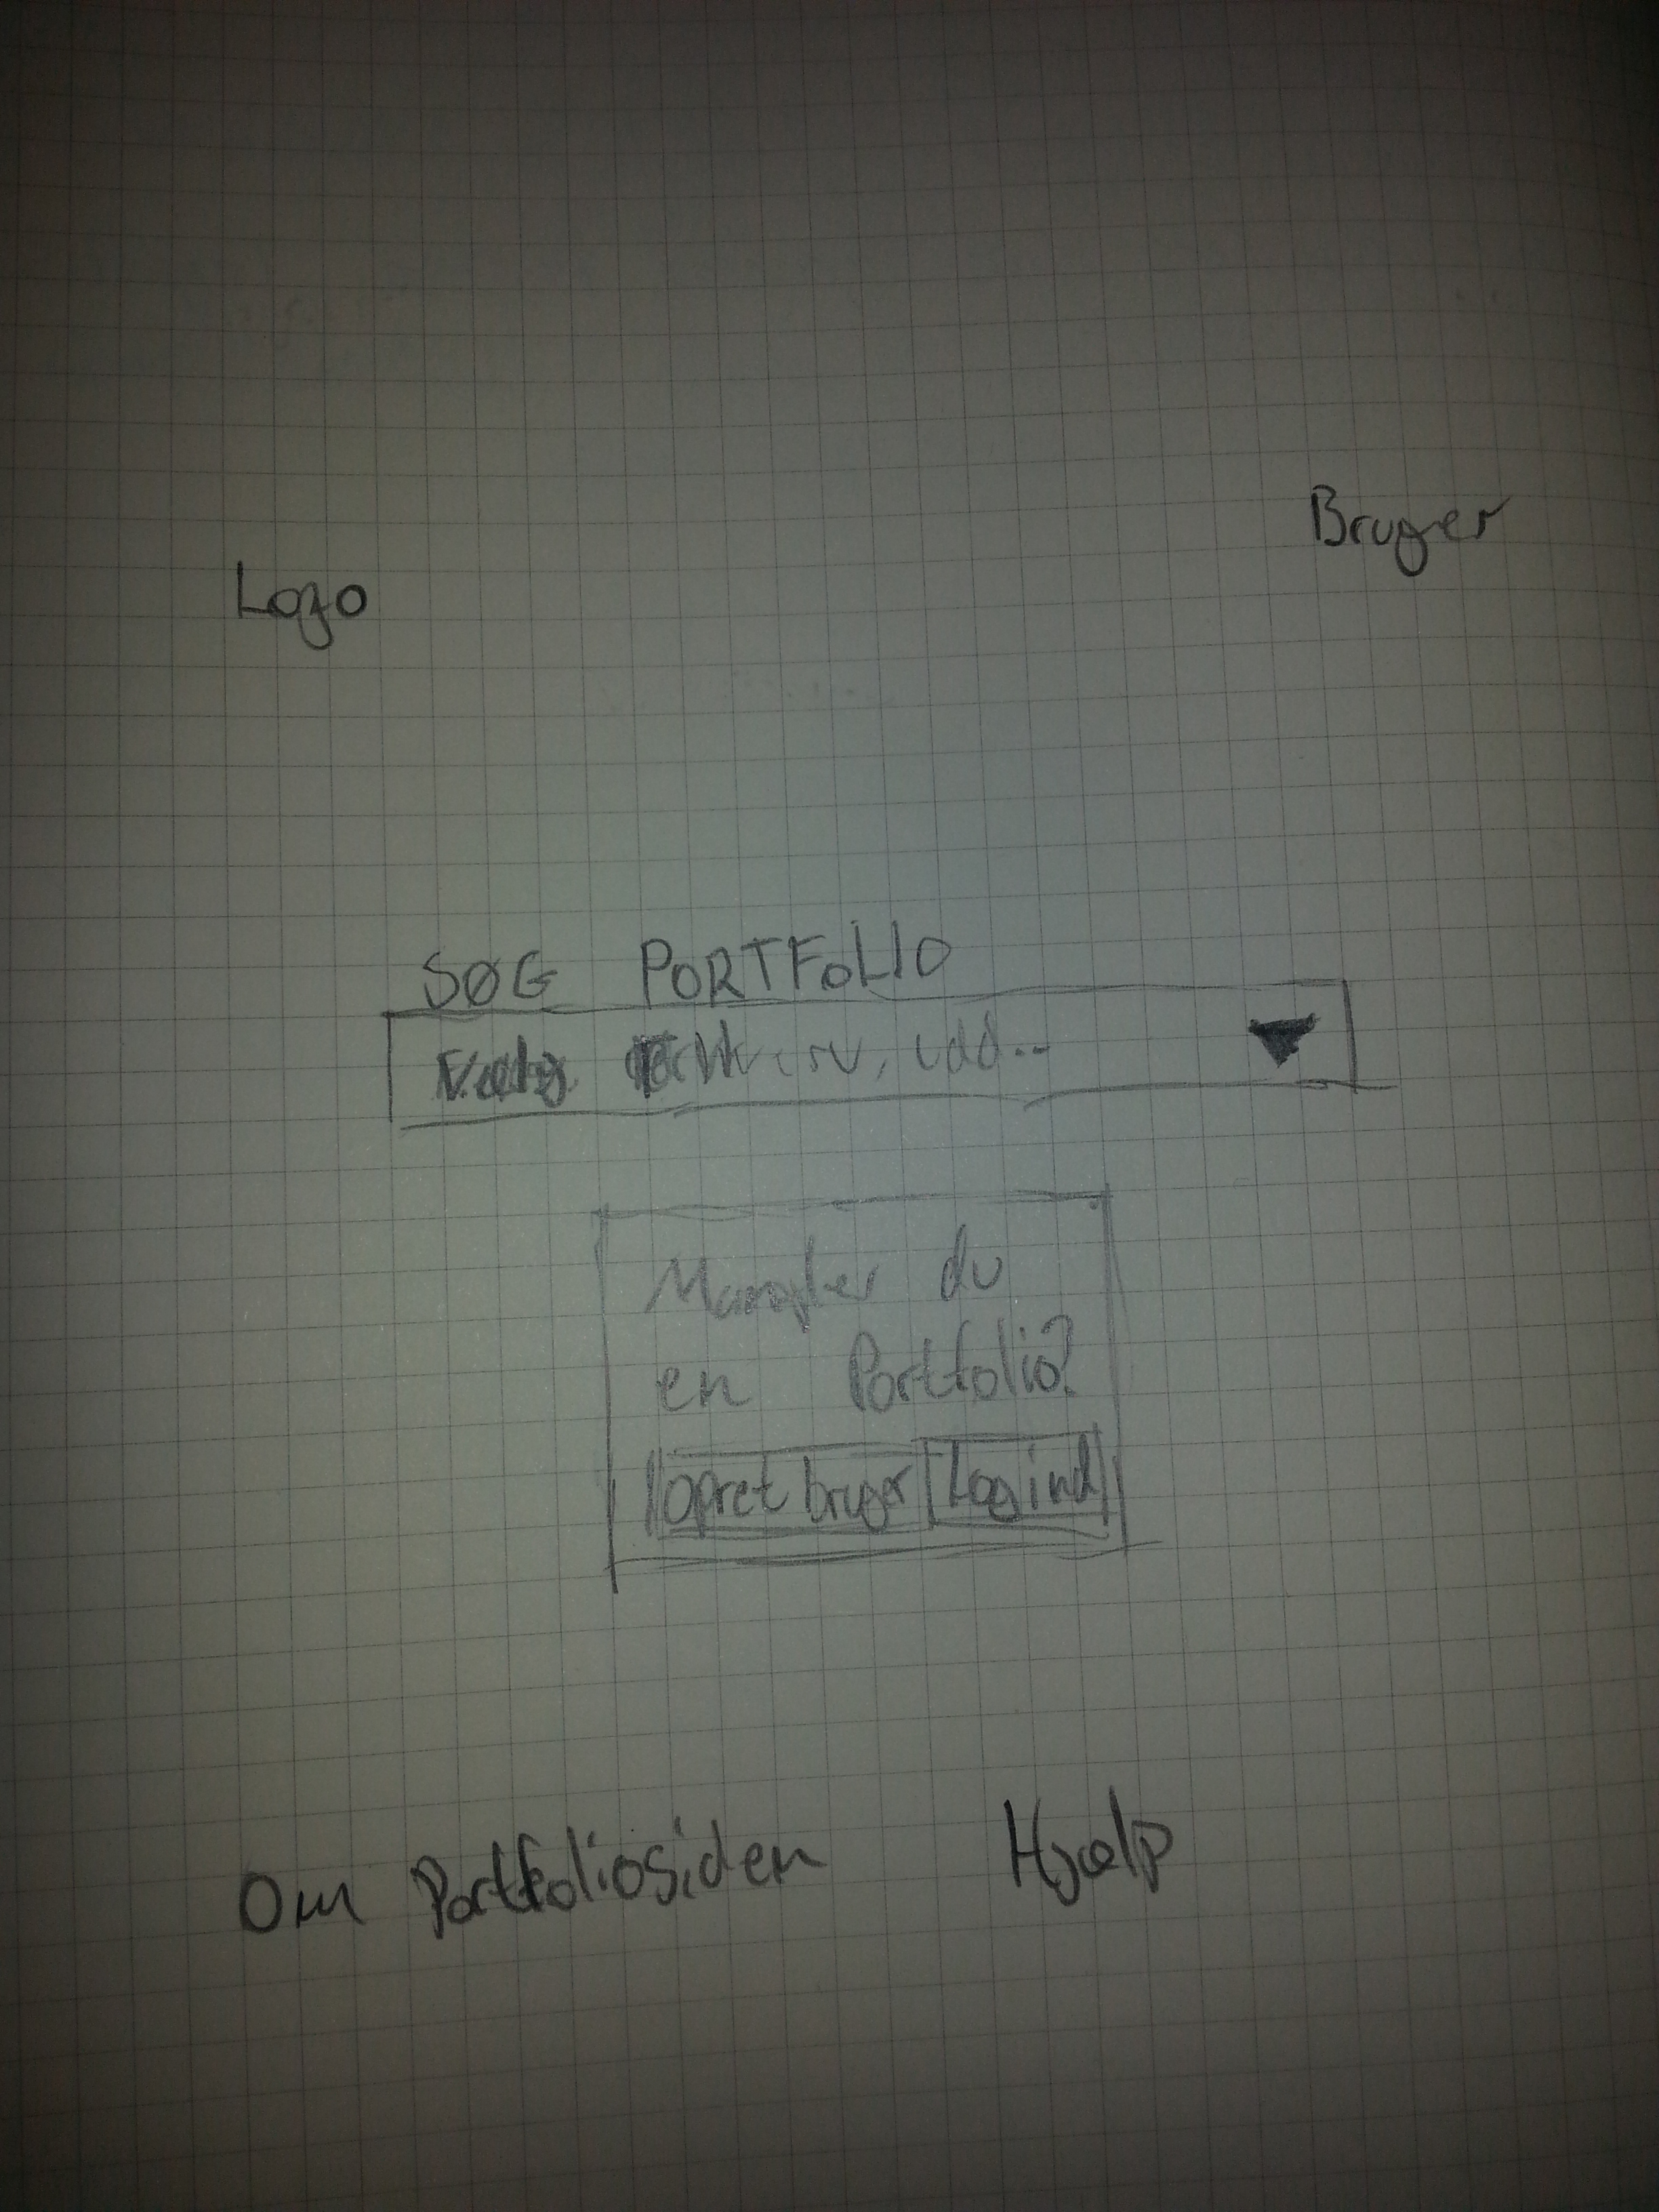
\includegraphics[width=\textwidth]{startside.jpg}
\caption{Startside hvor man kan søge på portfolier}
\end{figure}

\begin{figure}[H]
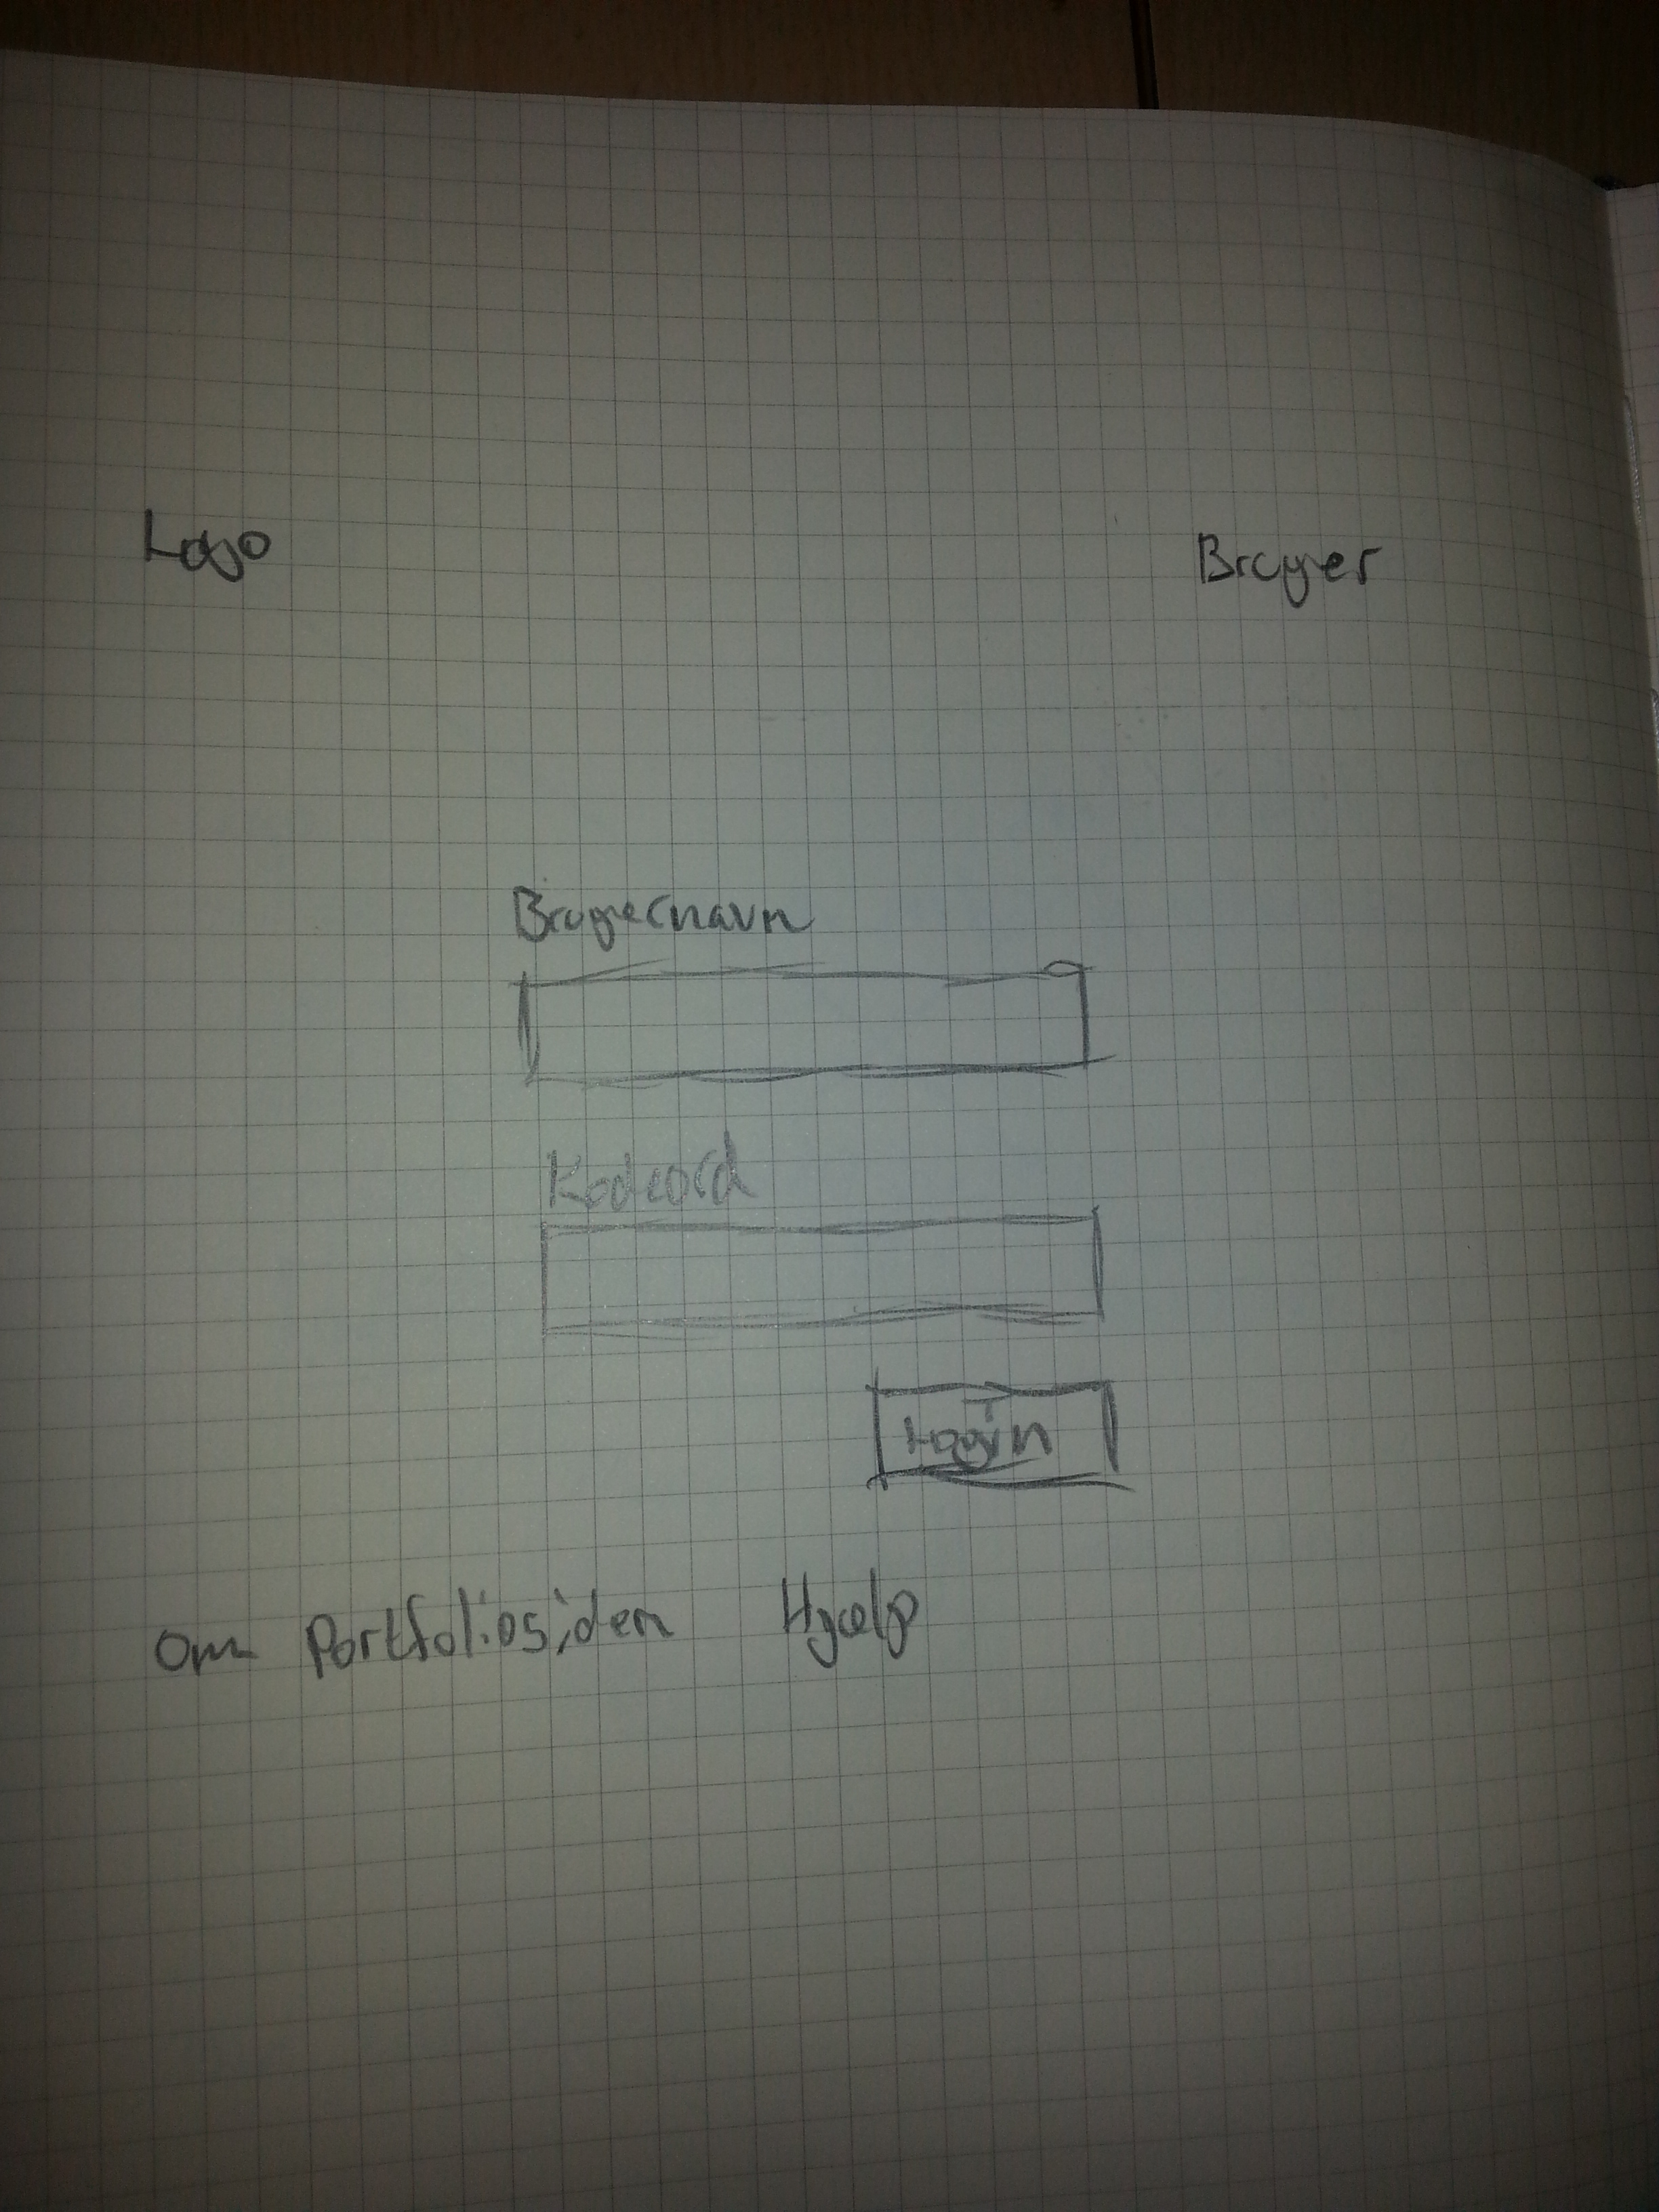
\includegraphics[width=\textwidth]{login.jpg}
\caption{Login screen hvis man har en bruger}
\end{figure}

\begin{figure}[H]
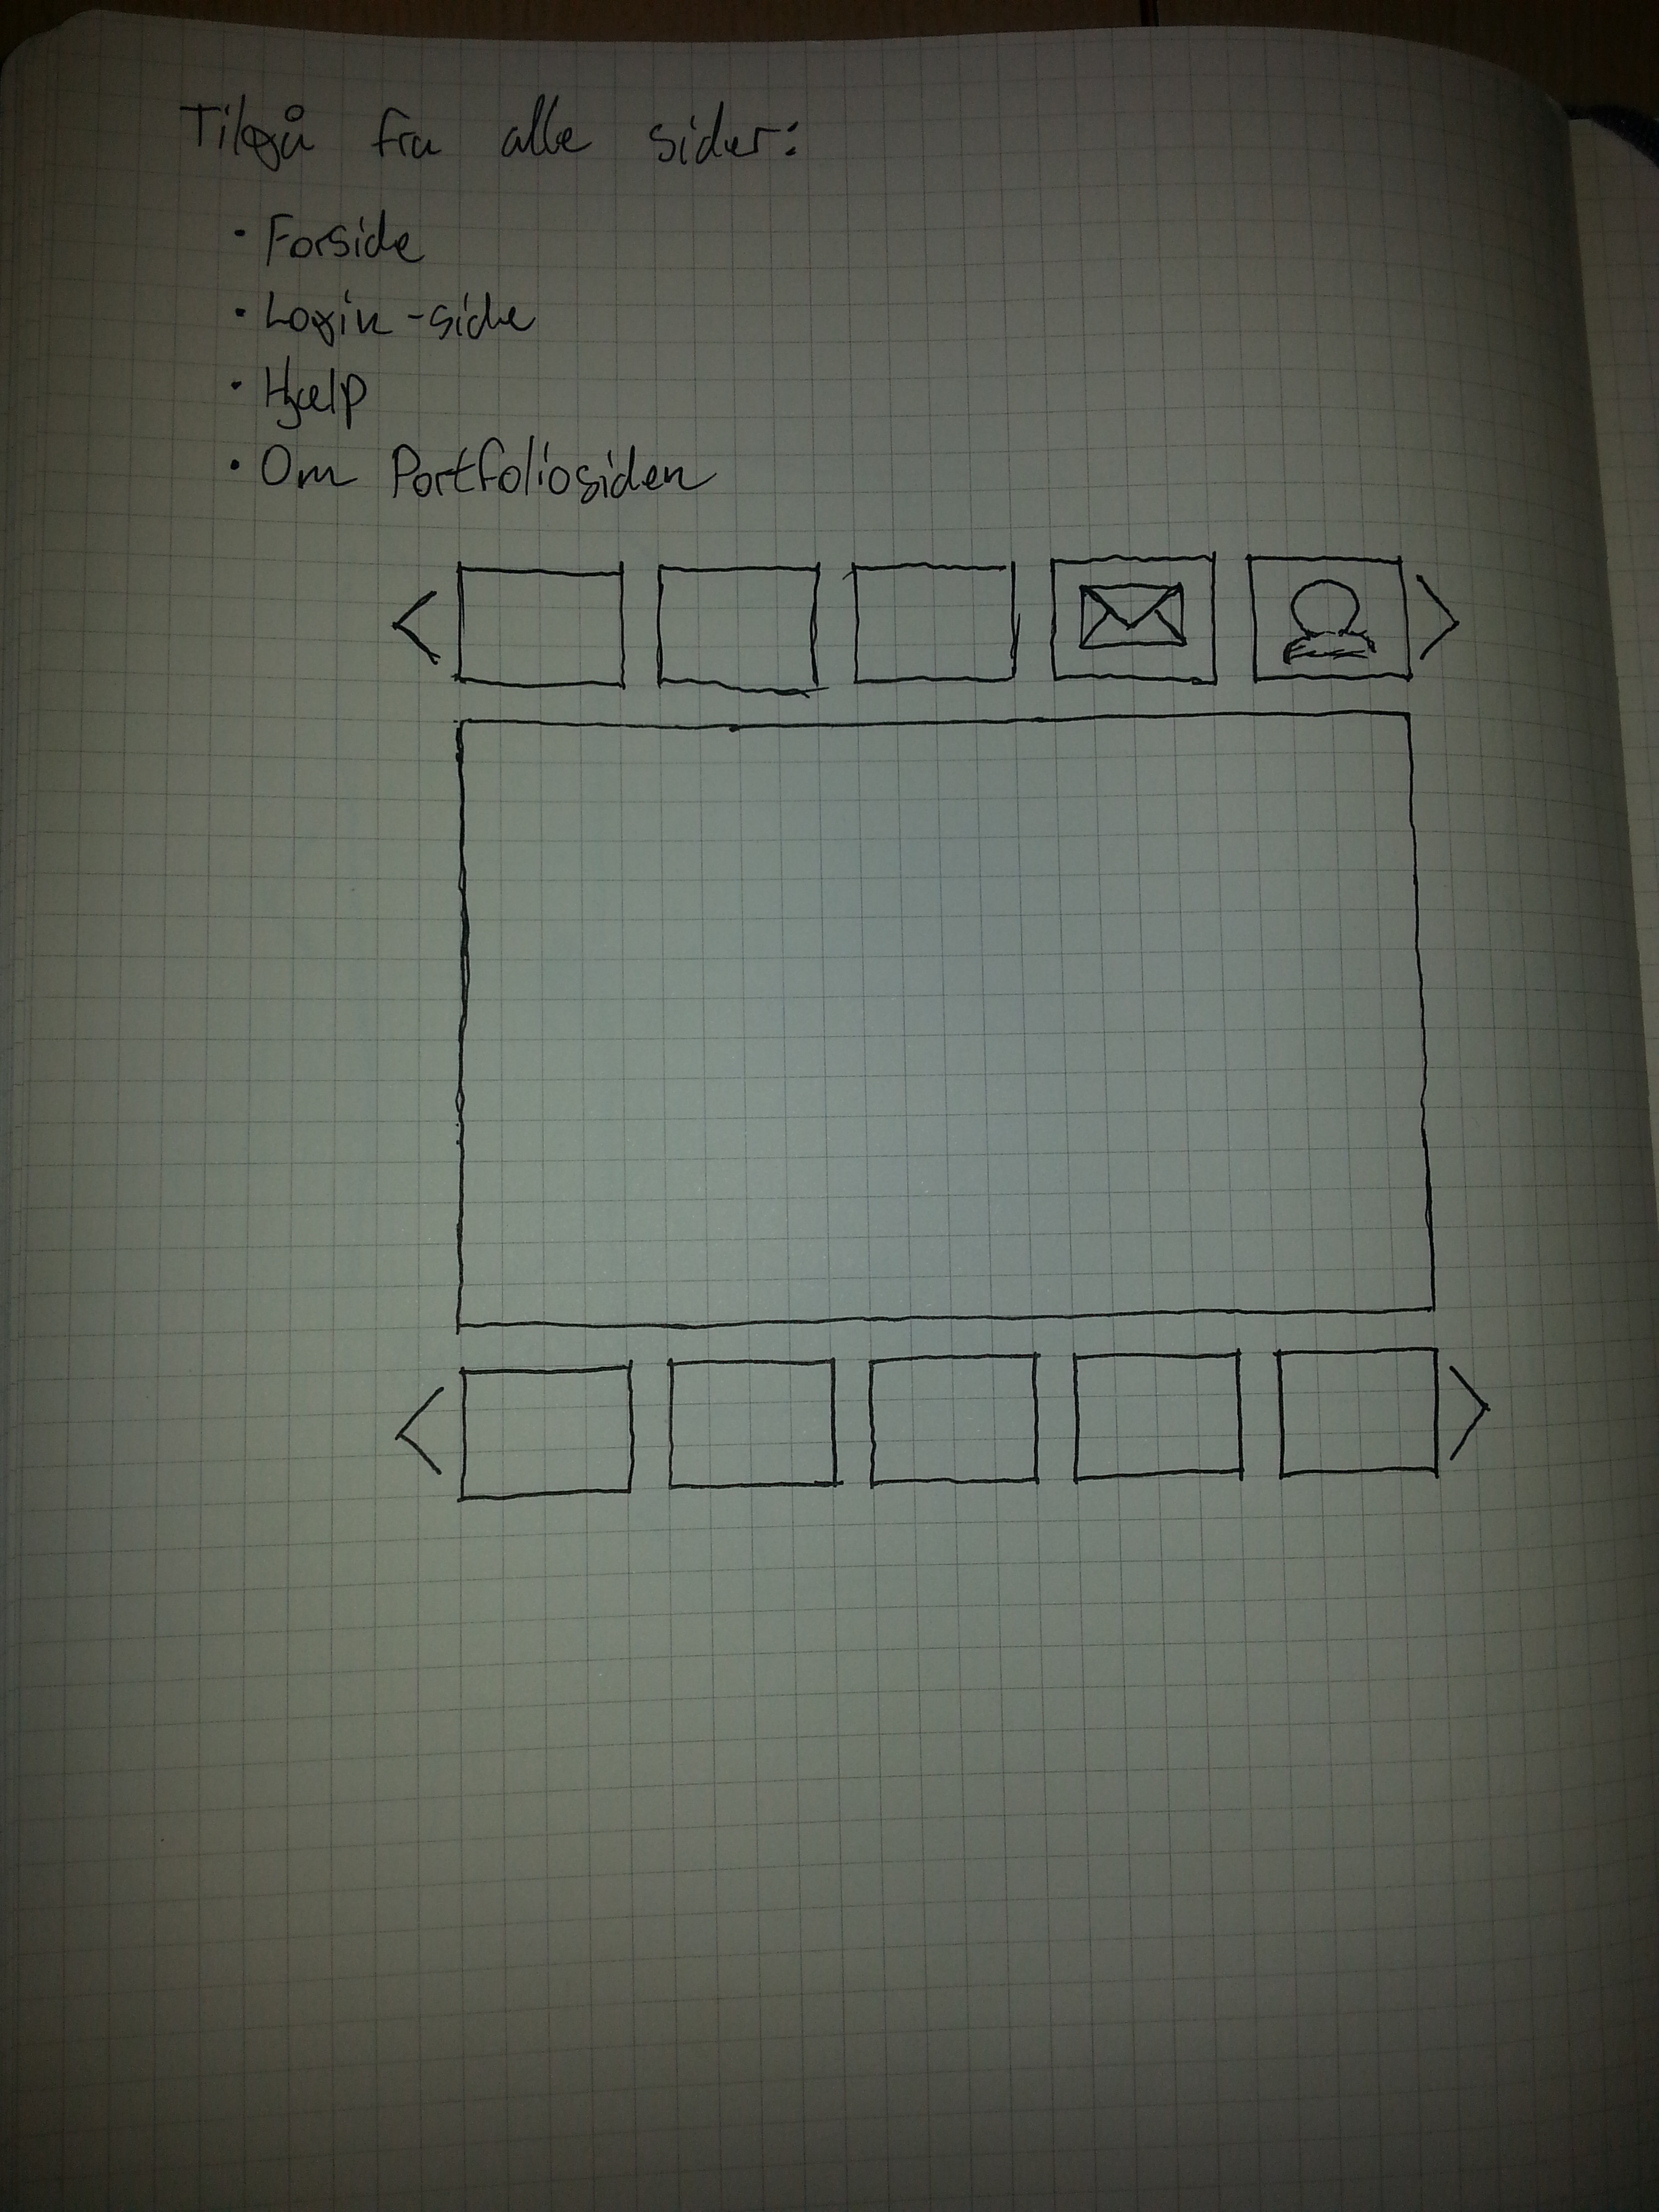
\includegraphics[width=\textwidth]{mainside.jpg}
\caption{Her ses portfolien, den vigtigste feature i vores løsning, hvor man kan tiløje og gennemse gemte projekter}
\end{figure}

Vi har desuden lavet en model af den databasestruktur vi har overvejet til projektet. Kort fortalt viser modellen hvordan alt data hænger sammen. Hver bruger kan registrere hvilket "område" og hvilken profession brugeren har (eller hvilket erhvervsmæssigt område brugeren er inden for). Derudover har hver bruger en eller flere portfolier tilknyttet, som hver har nogle projekter tilknyttet som dernæst har nogle "items" tilknyttet. Dette kunne for eksempel være billeder, videoer, tekst, m.v.

\begin{figure}[H]
	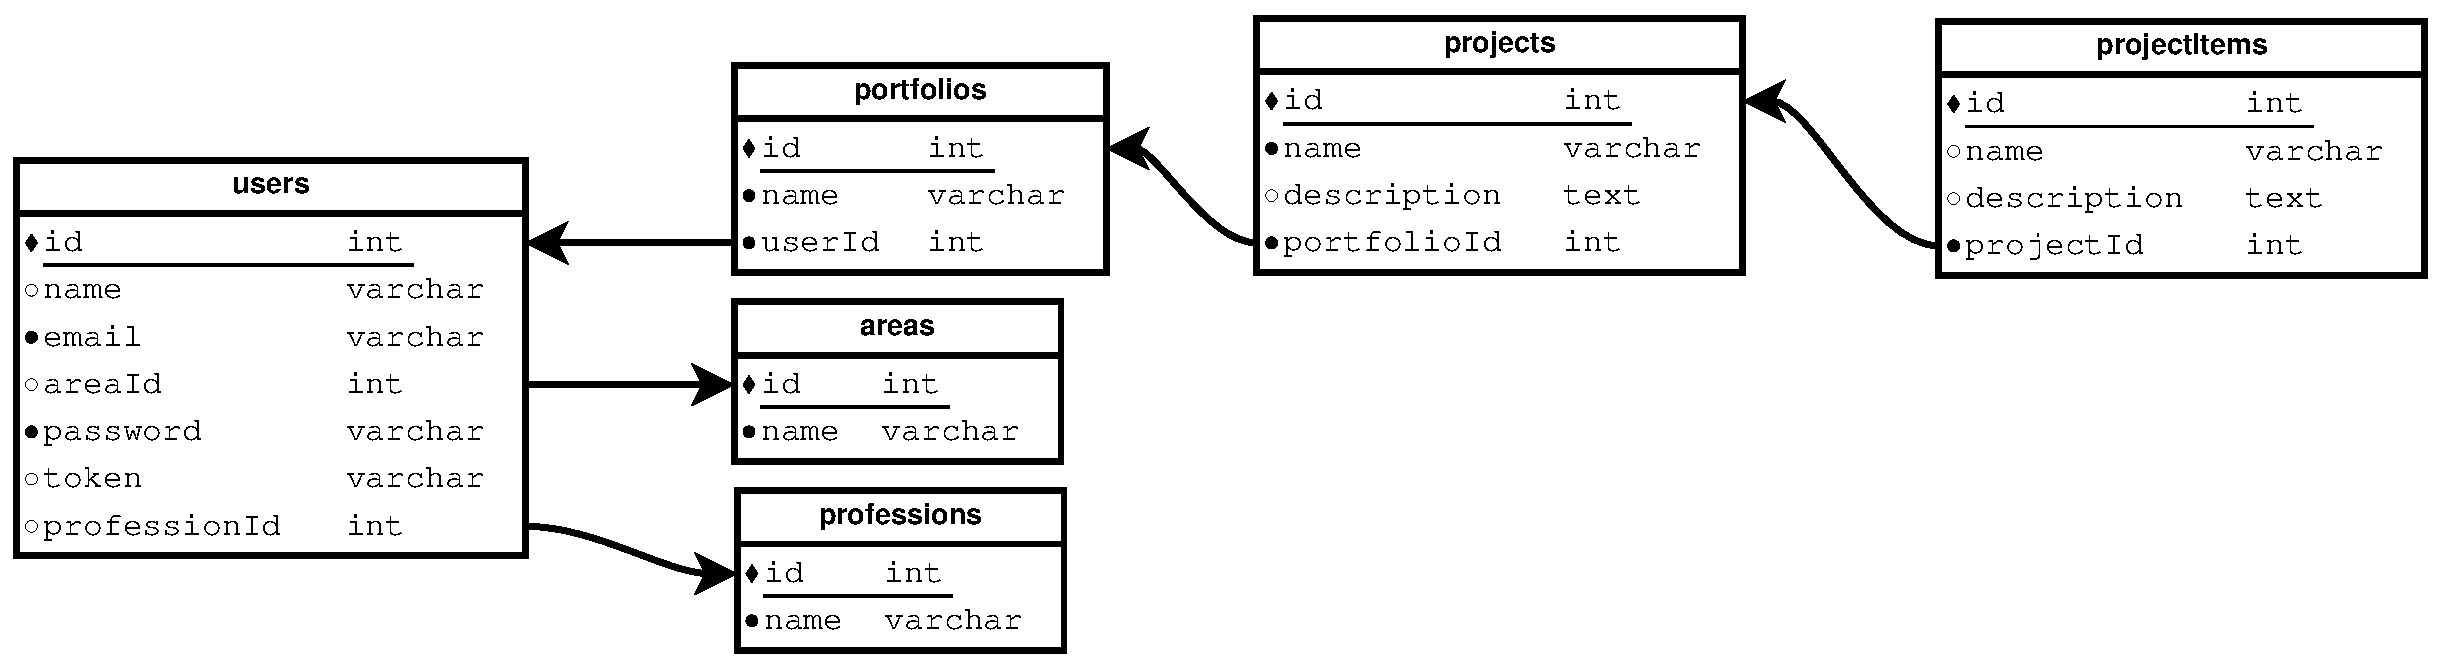
\includegraphics[width=\textwidth]{database.eps}
	\caption{Databasedesign over projektet}
\end{figure}

\section{Personas}
\subsection{Lisa, 24 år}
\begin{description}
	\item[Beskæftigelse] Designstuderende på Århus Universitet
	\item[Teknisk følelse/attitude] glad for teknologi, og fremadrettet design mæssigt.
\end{description}
\paragraph{Baggrund}\hfill\\Lisa er en frisk ung pige der til daglig studerer på universitet, og har en bred omgangskreds. Lisa drømmer om at kunne afslutte universitet og komme ud og prøve kræfter med erhvervslivet men har ikke rigtig lavet andet erhvervsmæsigt end at sidde ved kassen i fakta. Hun bor alene i byen uden andre.

\subsection{Henning, 22 år}
\begin{description}
	\item[Beskæftigelse] Webintegrater freelance arbejder
	\item[Teknisk følelse/attitude] høj teknisk viden.
\end{description}
\paragraph{Baggrund}\hfill\\Henning er en ung og udadvendt mand, hvis liv primært drejer sig om hans arbejde. Han beskæftiger sig med freelance design og programmering af hjemmesider, hovedsagligt for mindre virksomheder. Der er dog mange om buddet på markedet, og det er meget forskelligt fra måned til måned, hvor meget arbejde han kan få. Henning er dog for nyligt flyttet sammen med hans kæreste Gertrud som arbejder på McDonalds, og de er lige i stand til at få økonomien til at løbe rundt i de måneder Henning ikke kan få så meget arbejde.

\subsection{George, 38 år}
\begin{description}
	\item[Beskæftigelse] Selvstændig erhvervsdrivende med 2 ansatte
	\item[Teknisk følelse/attitude] Ikke særlig teknisk anlagt og gider ikke computere
\end{description}
\paragraph{Baggrund}\hfill\\
George er en travl middelaldrende mand som er født i Skotland og kommet til Danmark som ung. Han er uddannet arkitekt og har sit eget artitektfirma. George er meget ambitiøs og engageret i sit arbejde, men har det også med at være stædig, og hans firma har ofte svært ved at følge med udviklingen og konkurrenterne da han ikke gider at bruge tid på computere og teknologi. 

\subsection{Betina, 45 år}
\begin{description}
	\item[Beskæftigelse] Key Account Manager i HR afdelingen hos LEGO. \item[Teknisk følelse/attitude] bruger behov, med kurser i excel og word. Bruger computer på arbejde og derhjemme dagligt.
\end{description}
\paragraph{Baggrund}\hfill\\
Betina er en frisk dame i sin bedste alder arbejdsmæssigt, og har flair for mennesker som hendes arbejde hovedsageligt handler om. Hun er udadvendt og smilende, tager gerne en udfordring op og er ikke bange for det heller. Betina er bosat med sin mand og to børn, og har en et godt sundt familieliv.

\section{Test af prototyper}

Vi har valgt to brugere, som vi mener kunne have interesse i at bruge vores produkt, til at teste vores tre low fidelity prototyper. 

Den ene er en medstuderende, som er uddannet elektriker. Han har valgt at studere videre, da dagligdagen som elektriker var for uinspirerende, samtidig fik han ondt i sine knæ når vinteren kom nærmere og kulden trak til. Vi kalder denne testperson Mand.

Vores anden test person er en kvindelig ingeniøestuderende som beskæftiger sig rigtig meget med musik i sin hverdag. Hun har udgivet flere sange, og passer derfor godt som testperson til vores projekt. Vi kalder denne testperson Kvinde.


\subsection{Prototype 1}

\begin{figure}[H]
	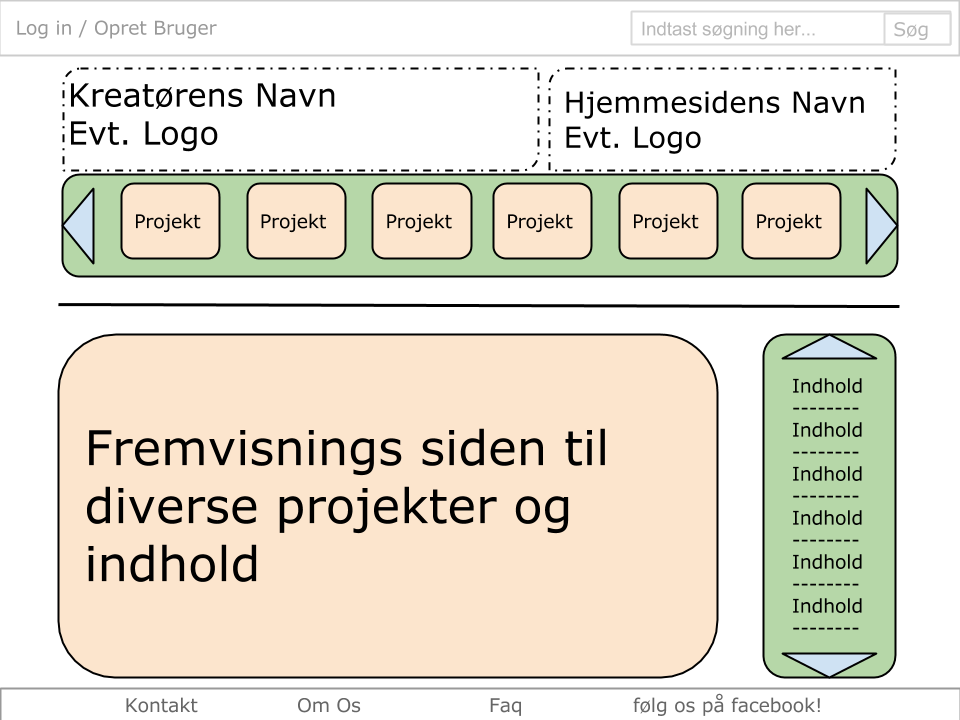
\includegraphics[width=\textwidth]{hjemmesidedesign1.png}
	
\end{figure}

\subsubsection{Mand}
Jeg synes det virker rigtig godt at mit eget navn har mere plads end hjemmesidens logo. Den lodrette liste til højre er lidt forvirrende. Det er dejligt at man bliver holdt på den samme side og ikke bliver kastet rundt mellem mange sider.

\subsubsection{Kvinde}
Jeg synes umiddelbart, at siden er nem at finde rundt på. Jeg synes det er fedt, at man kan få et logo op ved siden af sit navn. Det er svært at finde ud af hvilke menulinjer der gør hvad.\\\\
Ud fra indput fra vores testpersoner har vi lavet en liste med fordele og ulemper

\subsubsection{Fordele}

\begin{itemize}
	\item Let tilgængelig søgefunktion.
	\item Det fremgår tydeligt hvis portfolie man er inde på.
	\item Overskueligt og nemt at tilgå diverse funktioner.
\end{itemize}

\subsubsection{Ulemper}
\begin{itemize}
	\item Svært at finde et specifikt billede i et projekt med mange billeder. 
	\item Forvirrende med både horisontale og vertikale lister
	\item Manglende information om indholdet i projekterne
\end{itemize}

\subsection{Prototype 2}

\begin{figure}[H]
	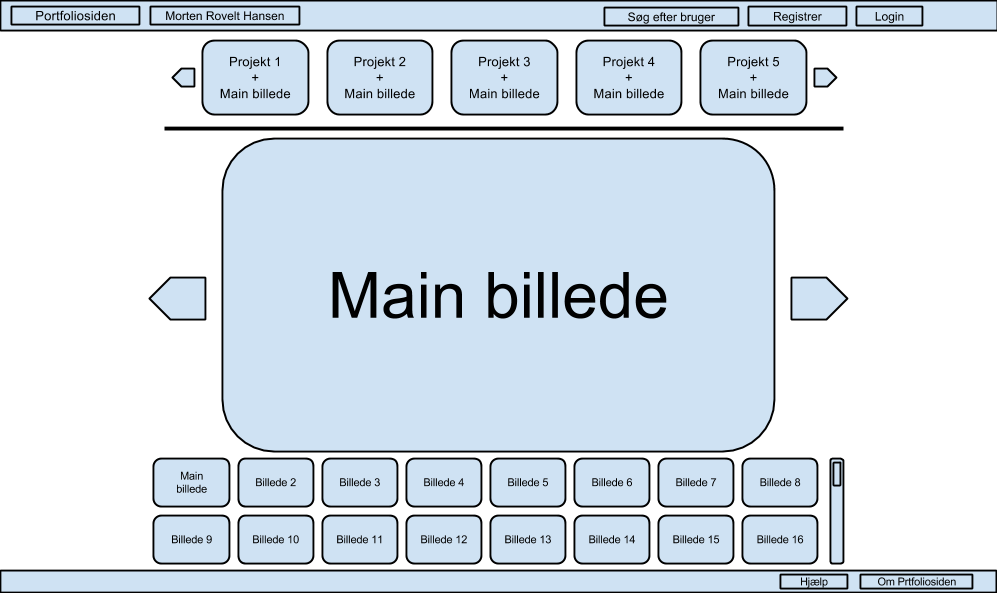
\includegraphics[width=\textwidth]{Prototype_1_not_logged_in.png}
\end{figure}

\begin{figure}[H]
	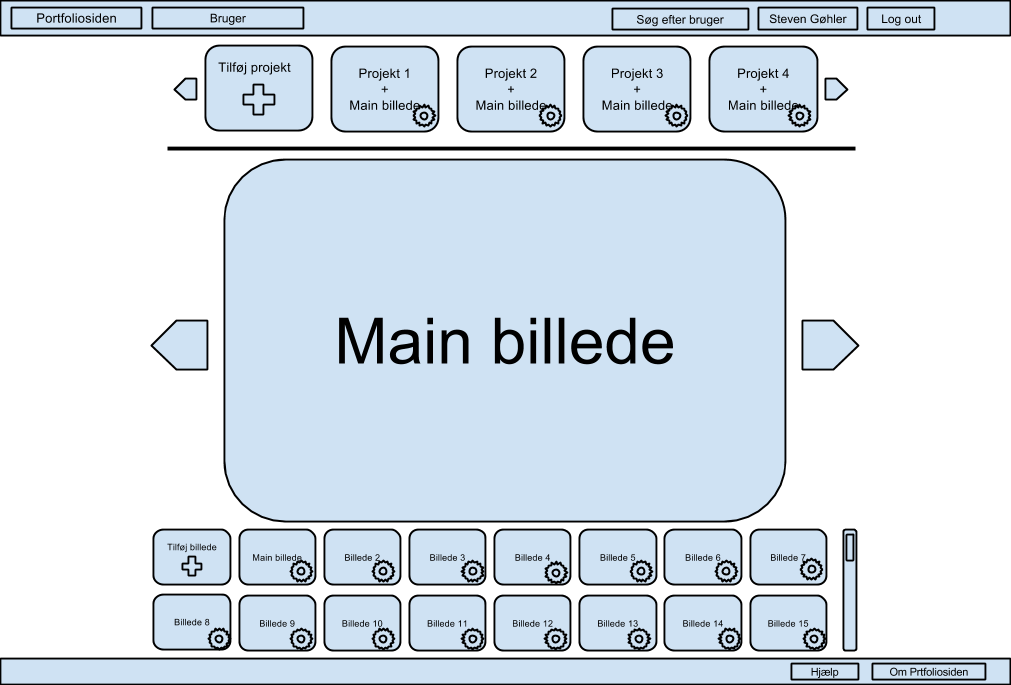
\includegraphics[width=\textwidth]{Prototype_1_logged_in.png}
\end{figure}

\subsubsection{Mand}
Jeg synes det er nemt at se alle billeder igennem i hvert projekt. Det virker meget ligetil at bruge, fordi der kun er to "lister" og så ét billede i fokus. Det kunne måske gøre siden bedre hvis man kunne skrive noget om hvert enkelt projekt.

\subsubsection{Kvinde}
Det hele er meget firekantet. Det er lidt irriterende, at man skal klikke ind på hvert projekt for at se hvad de indeholder. Jeg synes det er en god idé, at man kan redigere i rækkefølgen på billeder og projekter ved brug af tandhjulet. Samtidig synes jeg også det virker som en god måde at tilføje og slette billeder på.\\\\
Ud fra indput fra vores testpersoner har vi igen lavet en liste med fordele og ulemper


\subsubsection{Fordele}
\begin{itemize}
	\item Let tingængelig søgefunktion
	\item Simpelt og overskueligt
	\item Nemt at tilføje/slette projekter og billeder
\end{itemize}

\subsubsection{Ulemper}
\begin{itemize}
	\item For mange elementer på skærmen af gangen
	\item Scroll bar bliver muligvis et problem
	\item Manglende infirmation om inholdet i projekterne
\end{itemize}

\subsection{Prototype 3}

\begin{figure}[H]
	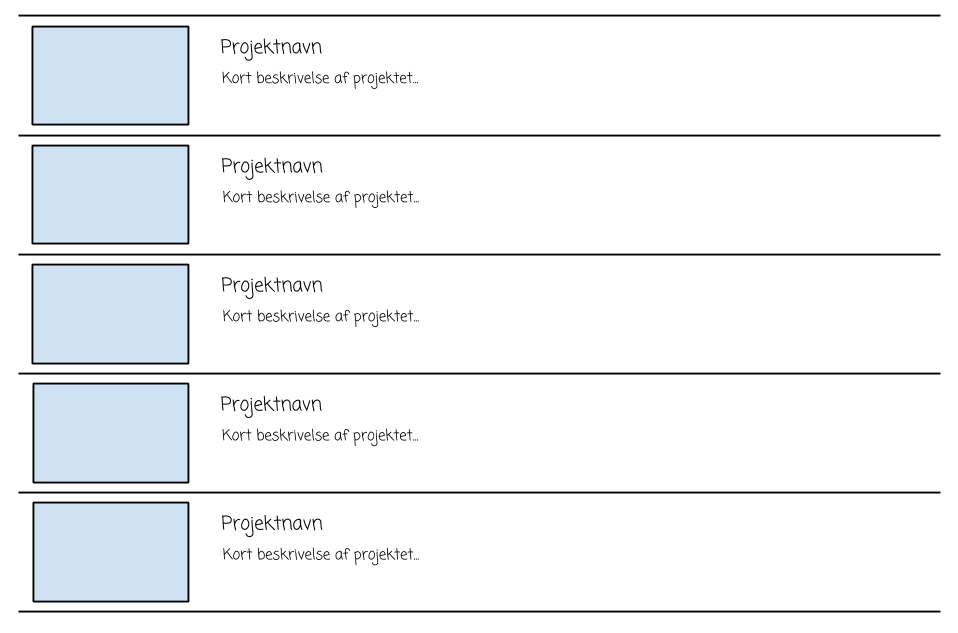
\includegraphics[width=\textwidth]{Sketch2_1.png}
\end{figure}

\begin{figure}[H]
	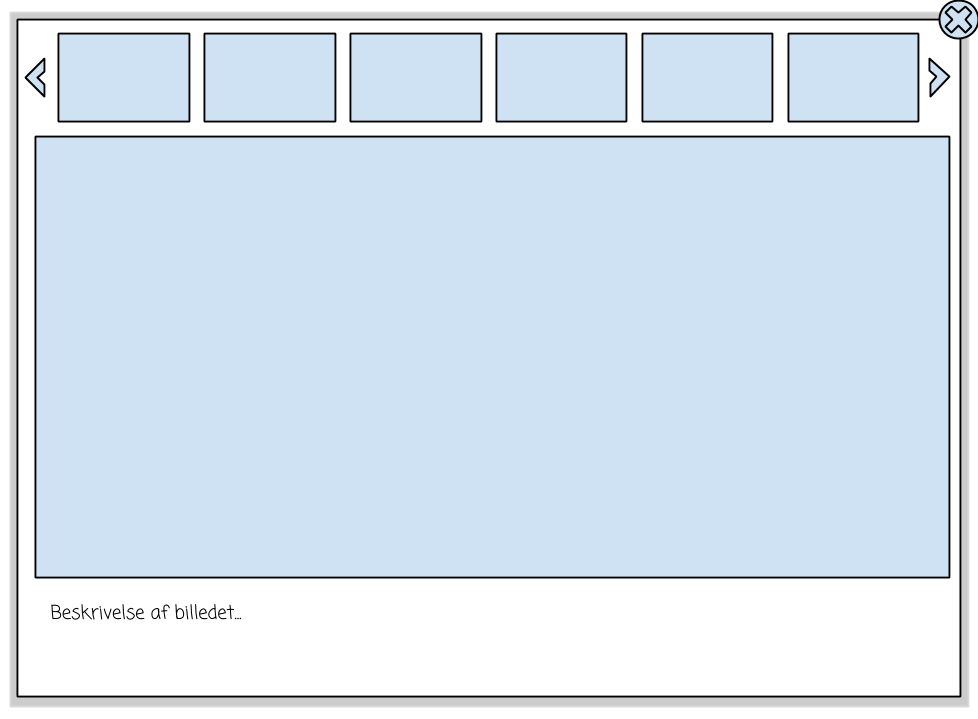
\includegraphics[width=\textwidth]{Sketch2_2.png}
\end{figure}

\subsubsection*{Mand}
Utrolig simpel og lækkert design. Meget let at se præcis hvad projektet indeholder. Jeg synes dettet er den bedste af de tre versioner jeg har set. 

\subsubsection*{Kvinde}
Jeg synes det er en rigtig god og overskuelig måde at stille det op på. Det er også rigtig let at se hvad projektet indeholder, på grund af den beskrivelses mulighed der er. Jeg synes dog, at det er lidt ærgeligt at man kommer ind på en ny side når man klikker ind på projektet.\\\\
Ud fra indput fra vores testpersoner har vi endnu engang lavet en liste med fordele og ulemper


\subsubsection{Fordele}
\begin{itemize}
	\item God information omkring projekterne
	\item Der er et minimum af elementer på siderne af gangen
\end{itemize}

\subsubsection{Ulemper}
\begin{itemize}
	\item Det er ikke nemt at tilgå et nyt projekt
\end{itemize}


\section{High fidelity prototype}

\subsection{Design valg}

Vi har valgt at designe vores high fidelity prototype ud fra den response vi har fået fra vore testpersoner. Vi var meget splittet i gruppen om, hvordan vi synes det ideale produkt skulle se ud. Vi besluttede os for at lave en low fidelity prototype hver, hvorefter vi bad to testpersoner om, at give os både positiv og negativ feedback på de tre varianter. Ud fra de fordele og ulemper fra feedbacken har vi besluttet at tage layoutet fra den tredje prototype, da det var det prototype layout begge testpersoner bedst kunne lide. Vi har altså en let overskuelig side med få elementer på hovede siden. Tilmed har vi også en god beskrivelse af hvert projekt ud på hovede siden. Når man opretter et projekt skal man samtidig vælge et main billede, som bliver vist på projektmappen på mainsiden. For at holde det simple layout, som begge testperson var rigtig glade for, har vi valgt at lave et pop-up vindue, hvor det valgte projekt bliver vist i. Dette pop-up vindue skal så vise de elemeter, som projektet indeholder, i toppe af pop-up vinduet. De skal fremvises med en menulinje med en pil i begge ender, til at bladre mellem hvert element. Man vælger et element ved, at klikke på det i menulinjen, hvorefter det valgte element (main billedet som standart) vil blive vist i stort format i midten af pop-up vinduet. Der vil tilmed være en beskrivelse af hvert element i bunden af pop-up vinduet, som eftertragtet af vores testpersoner.

\section{Evaluering}
Fremgangsmåden i den generelle proces af projektet er meget god, 
da man i forhold til en normal tilgang ville overse emner og aspekter
af det der er vigtigt både for udviklere og brugere. Dialogen med 
diverse testpersoner under udviklingen af selve prototyperne vi har været igennem, har været ideel i forhold til, at vores testpersoner rammer rigtigt på de focuspunkter vi under anden portefølje var i tvivl om, hvordan ville blive taget imod fra en brugerens side af. 
Synspunkterne som kommer til lys under en proces som denne er guld 
værd når man kigger tilbage på hvad man selv gerne vil have, og hvad
en potientiel bruger gerne vil have, da disse to ting finder sig ofte
at være meget forskellige. Løsningen vi er kommet frem til er blevet til et produkt der på sigt, kan udvikles til en rigtig god side, som vi er helt sikre på at folk i alt almindelighed vil bruge. Det er en super måde at tilføje noget ekstra til ens resumé udover de sædvanlige sociale medier, eller et håndskrevet dokument. Der er en bred vifte af muligheder i opsætningen på siden, og en meget fin overgang fra 
det visuelt gode ved en enkel side og den funktionelle del.
Efter det er sagt, er det heller ikke meningen at vores udarbejdelse skal ramme alle sociale klasser, men vi er specifikt gået efter en løsning der kan ramme folk der søger et let visuelt design, uden selv at have den viden der skal til for at sætte selve siden op, men bare vil ændre på de nøgleværdier der for enhver person gør deres side personlig.
Vores etnografi har hovedsageligt udspillet sig i brainstorms med udgangs-punkt i deltagerobservation af det individ vi havde udvalgt til at kigge og interagerer med vores prototyper, og denne fremgangsmetode er meget målrettet for vores projekt, og viste sig at være en gunstig metode.

\end{document}